\chapter{Oefeningen}

Dit hoofdstuk bevat de oefeningen die door het jaar heen gemaakt zullen worden. De lector zal je door het jaar heen helpen bij het maken met deze oefeningen. Indien je naast deze oefeningen graag nog extra oefeningen maakt, mag je natuurlijk altijd online nog extra oefeningen zoeken.

Voor sommige oefeningen moet je gebruik maken van bestanden die op voorhand beschikbaar gesteld zijn. Bij deze oefeningen zal dit telkens duidelijk vermeld staan.

\section{Conditionele Logica en Lussen}

\subsection{Maximum}

Schrijf een programma dat het maximum berekent van 10 getallen. Breid het programma uit zodat eerst gevraagd wordt hoeveel getallen de gebruiker gaat ingeven (in plaats van telkens 10 getallen te vragen).

\subsection{Even getallen}

Schrijf een programma dat het aantal even getallen berekent van 10 getallen. Breid het programma uit zodat eerst gevraagd wordt hoeveel getallen de gebruiker gaat ingeven (in plaats van telkens 10 getallen te vragen).

\subsection{Grootste verschil}

Bepaal in een reeks van 10 getallen het grootste verschil (d.w.z. het verschil tussen het grootste en het kleinste getal in de reeks). Breid het programma uit zodat eerst gevraagd wordt hoeveel getallen de gebruiker gaat ingeven (in plaats van telkens 10 getallen te vragen).

\subsection{Groter dan voorgaande}

Bepaal in een reeks van 10 getallen het aantal getallen dat groter is dan het voorgaande getal. Breid het programma uit zodat eerst gevraagd wordt hoeveel getallen de gebruiker gaat ingeven (in plaats van telkens 10 getallen te vragen).

\subsection{Piramide}

Karel wil een piramide maken van N hoog. De basis bestaat uit N blokjes en elke rij heeft exact 1 blokje minder. Figuur~\ref{fig:piramide} toont een voorbeeld bij N = 10. Het aantal benodigde blokjes om deze piramide te bouwen is 55.

\begin{figure}
\centering
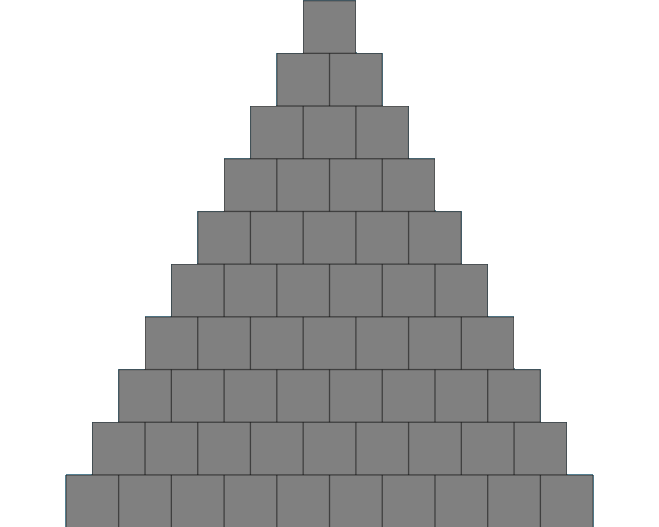
\includegraphics[scale=0.5]{Oefeningen/blokjes.png}
\caption{Een piramide met een basis van 10 blokjes}\label{fig:piramide}
\end{figure}

Schrijf een programma dat op basis van n (>= 1) berekent hoeveel blokjes Karel nodig heeft.

\subsection{Kubus}

Kleine Karel stapelt blokjes, en maakt daarbij een aantal kubussen. Hij maakt eerst een kubus van 1 blokje hoog (dat is dus 1 blokje op zichzelf). Daarnaast maakt hij een kubus van 2 blokjes hoog (en dus ook breed en diep), daarnaast een kubus van 3 blokjes hoog, enzovoorts, tot hij een hele reeks kubussen voor zich heeft staan.

Schrijf een programma dat het totale aantal blokjes berekent dat Karel nodig heeft om n kubussen te maken, die een oplopende hoogte hebben van 1 tot n.

\begin{tabular}{ p{5 mm} c c }
 & \textbf{Invoer} & \textbf{Uitvoer} \\
 & 1 & 1 \\
 & 2 & 9 \\
 & 3 & 36 \\
 & 6 & 441 \\
 & 7 & 784 \\
 & 57 & 2732409 \\
\end{tabular}

\subsection{Fibonacci}

De rij van Fibonacci is genoemd naar Leonardo van Pisa, bijgenaamd Fibonacci, die de rij noemt in zijn boek Liber abaci. In woorden is elk element van de rij steeds de som van de twee voorgaande elementen, beginnend met 0 en 1. De rij van Fibonacci (vaak ook reeks van Fibonacci genoemd) blijkt interessante eigenschappen en verbanden te bezitten met onder andere de gulden snede. De eerste elementen van de rij [1] zijn dan als volgt:

0, 1, 1, 2, 3, 5, 8, 13, 21, 34, 55, 89, 144, 233, 377, 610, 987, 1597, 2584, 4181, 6765, 10946, \ldots

Schrijf een programma dat het $N^{de}$ getal van fibonacci berekent.

\begin{tabular}{ p{5 mm} c c }
 & \textbf{Invoer} & \textbf{Uitvoer} \\
 & 1 & 0 \\
 & 3 & 1 \\
 & 10 & 34 \\
 & 15 & 377 \\
\end{tabular}

\subsection{Gespiekt}

In deze opgave moeten jullie een programma schrijven dat ons helpt om spiekende studenten te detecteren. De detectie zal hier gebeuren op basis van de plaats waar de studenten zitten. In onze situatie kan een student enkel spieken van een student die naast hem zit. Studenten die naast elkaar zitten en gelijkaardige punten hebben kunnen van spieken worden verdacht. Alle studenten zitten op \'e\'en lange rij. De eerste heeft plaats 1, de tweede plaats 2, enz. Aan het programma worden de punten van alle studenten van een examen gegeven volgens de plaats waar deze studenten zaten, dus eerst de punten van de student op plaats 1, dan de punten van de student op plaats 2, enz. Het programma moet als resultaat de 2 plaatsnummers geven waar het verschil tussen de punten van de studenten op die plaatsen het kleinst was. Indien er meerdere paren plaatsen voorkomen met een kleinste verschil, moet je enkel het eerste paar uitschrijven (volgens de gegeven rangschikking).

\paragraph{Invoer} Het eerste getal is het aantal studenten S dat aan het examen heeft deelgenomen (0 <=S <=1000). Daarna volgen S punten. Elk punt p is een geheel getal 0 <= p <= 20.

\paragraph{Uitvoer} Als het aantal studenten 0 of 1 is kan er niet worden gespiekt en moet de boodschap ``spieken kon niet'' gegeven worden. Anders moet de boodschap ``s1 en s2 zijn verdacht'' gegeven worden, waarbij s1 en s2 getallen zijn die de plaatsen aanduiden van de studenten die gespiekt kunnen hebben (kleinste verschil).

\paragraph{Kleine uitbereiding} Als het verschil tussen twee opeenvolgende punten 0 is, moet de boodschap ``s1 en s2 zijn zwaar verdacht'' gegeven worden. Hierbij zijn s1 en s2 getallen die de plaatsen aanduiden van de studenten die gespiekt kunnen hebben.

\begin{tabular}{ p{5 mm} c c }
 & \textbf{Invoer} & \textbf{Uitvoer} \\
 & 1 6 & spieken kon niet \\
 & 4 12 13 8 16 & 1 en 2 zijn verdacht \\
 & 5 10 10 14 14 10 & 1 en 2 zijn zwaar verdacht \\
\end{tabular}

\subsection{Decimaal naar binair}

Schrijf een stukje code om van een positief decimaal getal de binaire equivalent te berekenen (zie cursus computersystemen p. 11).

\subsection{Binair naar decimaal}

Schrijf een stukje code om van een positief binair getal de decimale equivalent te berekenen.

\section{RoboProg}

In deze oefeningen ga je een robotje besturen aan de hand van JavaScript-commando's. Het robotje verstaat en aantal elementaire commando's (deze worden hieronder uitgelegd), en jij moet er voor zorgen dat het robotje zijn doel bereikt. Hiervoor kan je, naast de commando's die de robot begrijpt, natuurlijk ook gebruik maken van JavaScript-functionaliteit zoals iteraties (for, while) en selecties (if).

De commando's die de robot begrijpt kan je aanspreken door de volgende methodes op te roepen:

\begin{itemize}
\item \textbf{turnRight();}	Draai de robot 90 graden naar rechts
\item \textbf{turnLeft();}	Draai de robot 90 graden naar links
\item \textbf{wallAhead();}	Geeft de waarde true terug indien er een muur voor de robot staat, of false in het andere geval
\item \textbf{wallOnLeft();}	Geeft de waarde true terug indien er een muur links van de robot staat, of false in het andere geval
\item \textbf{wallOnRight();}	Geeft de waarde true terug indien er een muur rechts van de robot staat, of false in het andere geval
\item \textbf{moveForward();} Beweegt de robot \'e\'en vakje vooruit (let op: indien je deze methode oproept terwijl er een muur voor de robot staat, dan gaat de robot stuk!)
\item \textbf{out();}		Geeft de waarde true terug indien de robot de eindstaat bereikt, of false in het andere geval
\item \textbf{mark();}		Markeert de tegel waar de robot op staat
\end{itemize}

De robot moet een aantal opdrachten uitvoeren. Elke opdracht staat beschreven in een HTML-bestand dat je verder moet aanvullen. De opdrachten staan gerangschikt van gemakkelijk naar moeilijk.

\subsection{ZoekMuur.html}

Schrijf een algoritme dat de robot naar een muur doet rijden. Hij moet halt houden op een vakje dat grenst met een muur. De robot begint altijd op een random positie.

\subsection{ZoekHoek.html}

Schrijf een algoritme dat de robot naar een hoek doet rijden. De robot begint altijd op een random positie.

\subsection{TekenP.html}

Schrijf een algoritme dat de letter 'P' tekent op het bord. Hiervoor kan je de mark()-methode gebruiken. De P moet zes vakjes hoog zijn en drie vakjes breed. De robot begint altijd op dezelfde plaats (en dezelfde ori\"entatie). Opgelet: nadat je de P getekend hebt, zal je geen automatische bevestiging krijgen dat je opdracht geslaagd is! Je moet dus zelf kijken of de output van de robot correct is.

\subsection{Spiraal.html}

Schrijf een algoritme dat de robot naar het midden van de spiraal leidt. Werk dit algoritme twee keer uit: eenmaal door gebruik te maken van enkel for-lussen, een tweede keer door gebruik te maken van enkel while-lussen. De robot begint altijd op dezelfde plaats (en dezelfde ori\"entatie).

\subsection{ZoekUitgang1.html}

De robot begint altijd op een random plaats in een random-gegenereerde kamer met \'e\'en uitgang. Schrijf een algoritme dat de robot naar de uitgang leidt.

\subsection{ZoekUitgang2.html}

De robot begint altijd op een random plaats in een random-gegenereerde kamer met \'e\'en uitgang. Het verschil met de vorige oefening is dat de kamer nu niet meer rechthoekig is. Schrijf een algoritme dat de robot naar de uitgang leidt.

\subsection{TekenPiramide.html}

Schrijf een algoritme dat een piramide tekent op het bord. De piramide heeft een basis van 10 blokjes, en per rij omhoog gaan er twee blokjes af. De robot begint altijd op dezelfde plaats (en dezelfde ori\"entatie).

\subsection{ZoekIngang.html}

De robot begint altijd op een random plaats buiten een random-gegenereerde kamer. Schrijf een algoritme dat de robot naar binnen loodst.

\section{Functies}

\subsection{BMI}

Schrijf een functie `berekenBMI' die het BMI van een persoon berekent, aan de hand van twee variabelen: lengte (in meter) en massa (in kilogram). De berekening gaat als volgt:

$BMI = \frac{massa}{lengte^2}$

Schrijf een stuk code die deze functie gebruikt. De code moet de lengte en de massa vragen, en zal dan aangeven of de gebruiker gezond is (BMI tussen 18.5 en 25), ondergewicht heeft (BMI < 18.5), overgewicht heeft (BMI tussen 25 en 30), of obees is (BMI > 30).

\subsection{Statistiek}

Schrijf een functie die de (wiskundige berekening) `faculteit' berekent. De faculteitoperatie wordt als volgt berekend:

$x! = x \times (x-1) \times \ldots \times 1$

Bijvoorbeeld, $3! = 3 \times 2 \times 1 = 6$. Let op: $0! = 1$.

Schrijf een tweede functie die berekent op hoeveel manieren k elementen kunnen gekozen worden uit n elementen. Dit kan berekend worden op de volgende manier:

$\binom{n}{k} = \frac{n!}{k!(n-k)!}$

Schrijf een stuk code die aan de gebruiker invoer vraagt voor de getallen n en k, en dan het resultaat toont.

\subsection{Som van Cijfers}

Schrijf een functie die de cijfers van een getal optelt (bijv. De invoer 123 geeft als resultaat 6).

Gebruik deze functie om een nieuwe functie te schrijven die hetzelfde doet, maar blijft doorgaan totdat het resultaat strikt kleiner dan 10 is. Bijvoorbeeld, de invoer 987 geeft als resultaat 24, wat groter dan 10 is. Op dit getal wordt de functie weer opgeroepen, wat het resultaat 6 oplevert. Dit is kleiner dan 10 en is dus het eindresultaat.

\subsection{ROT-13}

De Romeinen gebruikten reeds een primitieve vorm van encryptie om er voor te zorgen dat berichten niet (of toch moeilijker) gelezen konden worden mochten ze in vijandelijke handen vallen. De versleuteling was eenvoudig: elke letter werd vervangen door een andere letter uit het alfabet. Zo wordt het bericht omgevormd tot op het eerste zicht onleesbare tekst.

Een moderne variant van dit algoritme is ROT-13. Elke letter uit het alfabet wordt vervangen door een letter die 13 plaatsen verder in het alfabet staat.

\texttt{Originele letter: a b c d e f g h i j k l m n o p q r s t u v w x y z}

\texttt{Resultaat:        n o p q r s t u v w x y z a b c d e f g h i j k l m}

Zo wordt de tekst ``de kat krabt de krollen van de trap'' na versleuteling ``qr xng xenog qr xebyyra ina qr genc''. Schrijf een stuk code die dit ROT-13-algoritme implementeert. Hieronder vind je de beschrijving van enkele functies die nuttig kunnen zijn om dit probleem uit te werken. (Ter herinnering: `a' heeft de ASCII-waarde 97)

\textbf{text.length()} kan opgeroepen worden op een variabele van het type `string' en geeft het aantal karakters terug waaruit de string bestaat.

\textbf{text.charCodeAt(positie)} kan opgeroepen worden op een variabele van het type `string' en geeft de ASCII-waarde terug van het karakter op de opgegeven positie. Let op: het eerste karakter van de string heeft positie 0!

\textbf{String.fromCharCode(asciiWaarde)} converteert de opgegeven ASCII-waarde naar een string van lengte 1 die dat karakter voorstelt.

\subsection{Vierkanten}

Kareltje tekent op de grond een vierkant met zijde \texttt{zijde1} cm, hij tekent vervolgens in dit vierkant telkens een ander vierkant waarvan de oppervlakte precies de helft is van het laatst getekende vierkant. Hoeveel vierkanten zal Karel tekenen als de zijde van het laatste vierkant hoogstens \texttt{zijde2} cm groot is. (\texttt{zijde1} en \texttt{zijde2} worden ingelezen)

\subsection{Converteer}

Schrijf een stuk code dat een getal converteert van de ene getalvoorstelling naar de andere. Bijvoorbeeld, de functie kan als invoer het getal 110010 krijgen, de getalvoorstelling van dit getal (in dit geval binair, dus de waarde 2) en het getalsysteem waarin de uitvoer moet gezet worden (bijv. het getal 8, om aan te geven dat de uitvoer een octaal getal moet zijn).

Zo kan de functie opgeroepen worden als volgt:
\begin{center}
\texttt{converteer(110010, 2, 8);}
\end{center}
Wat als resultaat het getal 62 oplevert (dit is de overeenkomstige octale voorstelling van het binaire getal 110010). De getalvoorstellingen die mogen opgegeven worden liggen tussen 2 en 10 (dus van binair tot decimaal).

Schrijf een stuk code dat je functie test. Controleer dat de berekening correct gebeurt!

\subsection{Konijnen Kweken}

Bij een fout gelopen experiment van dr. Cedric Parker-Powell (P.P. voor de vrienden) werden zijn proefkonijnen blootgesteld aan een overdosis radioactieve straling. Op het eerste zicht leek er niets mis met de konijnen, maar bij nader onderzoek blijkt hun reproductiesysteem grondig ontregeld: dat verloopt nu in fasen.

Stel dat er op een gegeven ogenblik n mutantkonijnen in het hok zitten. Als n even is, dan gaan de konijnen in hongerstaking tot er nog maar de helft over is. Als n oneven is, dan kweken ze bij tot ze aangegroeid zijn tot $3n + 1$ konijnen. Dit proces herhaalt zich natuurlijk tot er nog maar 1 konijn over is, ze moeten met 2 zijn om zich voor te planten!

P.P. weet nu al dat zijn konijnenhok niet groot genoeg is om alle konijnen te herbergen. Kan jij hem vertellen op welk maximaal aantal konijnen hij voorzien moet zijn?

Let op, de konijnpopulatie vertoont rare sprongen. Bijvoorbeeld, vertrekkende van 7 konijnen, worden achtereenvolgens de volgende aantallen doorlopen:

7 22 11 34 17 52 26 13 40 20 10 5 16 8 4 2 1

Het hok moet in dit geval dus voorzien zijn op 52 konijnen!

Om P.P. te helpen zal je het initi\"ele aantal konijnen moeten weten, maar al wat P.P. je kan vertellen is dat het ergens in het interval $[l; u]$ ligt.

\paragraph{Probleem} Wat is het grootste aantal konijnen dat er op een willekeurig moment kan voorkomen, gegeven dat het initi\"ele aantal konijnen in het interval $[l; u]$ ligt?

\paragraph{Invoer} De invoer bestaat uit twee getallen: de ondergrens l en de bovengrens u, waarbij l groter of gelijk is aan 1 en u kleiner of gelijk aan 500.

\paragraph{Uitvoer} De uitvoer bestaat uit \'e\'en natuurlijk getal m dat het maximale aantal konijnen aangeeft.

\subsection{Top 100}

Een radiozender wenst op het einde van het jaar een top 100 uit te zenden. Hiervoor wordt er aan de luisteraars gevraagd om een favoriete lijst op te stellen van songs. Dit resulteert een lijst van 100 liedjes waarbij op 1 het meest populaire liedje staat. Voor elke liedje beschik je over informatie met betrekking tot het aantal minuten (geheel) dat het liedje duurt. Deze honderd liedjes moeten gespeeld worden in blokken van 55 minuten, aangezien er elk uur een pauze van 5 minuten wordt voorzien voor reclamespots.

Uiteraard passen de liedjes niet altijd volledig binnen 1 blok. We mogen geen liedjes splitsen over 2 blokken. Dit betekent dat of de resterende tijd moet volgepraat worden door de DJ of dat een liedje niet volledig kan gespeeld worden. Voor beide oplossingen worden er strafpunten per minuut voorzien.

Bereken voor een gegeven aantal liedjes, gegeven lengte van een blok, gegeven strafpunt per minuut voor het niet spelen van een liedje, gegeven strafpunt  per minuut voor tijd volgepraat door de DJ en gegeven de lengte in minuten van de N liedjes, de minimale strafpunten.

\begin{tabular}{ p{5 mm} l l }
 & \textbf{Invoer} & \textbf{Voorbeeld 1} \\
 & Aantal lidjes: & 10 \\
 & Aantal minuten per blok: & 25 \\
 & Strafpunt per minuut dat een liedje niet wordt gespeeld: & 2 \\
 & Strafpunt per minuut dat de DJ de tijd moet volpraten: & 1 \\
 & N getallen, die het aantal minuten per liedje voorstelt: & 8 7 3 5 4 2 9 4 3 4 \\
 & & \\
 & \textbf{Uitvoer} & \\
 & Minimaal aantal strafpunten (1 getal): & 4 \\
\end{tabular}

\section{Recursie}

\subsection{Faculteit}

Schrijf een recursieve methode fac die \'e\'en parameter n heeft en als resultaat $n!$ teruggeeft. Maak hierbij gebruik van de recursieve definitie die in de cursus vermeld staat. Schrijf ook een tweede methode dubbelfac die \'e\'en parameter $n$ heeft en als resultaat de dubbelfaculteit teruggeeft (ook genoteerd als: $n!!$). Enkele voorbeelden van dubbelfaculteit: $9!! = 9.7.5.3.1, 8!! = 8.6.4.2$.

\subsection{Grootste Gemene Deler}

Schrijf een recursieve methode ggd die twee parameters a en b heeft en als resultaat de grootste gemene deler van a en b teruggeeft. Gebruik voor deze berekening het algoritme van Euclides.

\subsection{Fibonacci}

Schrijf een recursieve methode fib die een parameter n heeft en als resultaat het n-de Fibonacci-getal teruggeeft. Je kan hiervoor gebruik maken van de recursieve definitie die in de cursus vermeld staat (en dus bij de berekening van fib(n) een recursieve oproep doen voor fib(n-1) en fib(n-2)). Kan je het algoritme iets verbeteren door in plaats van twee recursieve oproepen te doen slechts \'e\'en recursieve oproep te doen?

\subsection{Hanoi}

Test het algoritme van de torens van Hanoi op de PC en zorg er voor dat je begrijpt hoe het werkt. Gebruik hiervoor de bestanden `hanoi.html' en `hanoi.js'. Teken op papier de verschillende stappen die het algoritme zal doorlopen indien we beginnen met 3 schijven op de eerste paal.

\subsection{Permutaties}

Een getal x is een permutatie van een ander getal y wanneer alle cijfers van x exact evenveel voorkomen in getal y en omgekeerd. Schrijf een recursieve methode isPermutatie(x, y) die nagaat of x een permutatie is van y.

Voorbeeld: 12345  en 51432 zijn permutaties, 1123 en 1233 zijn geen permutaties

\subsection{Strings}

Schrijf code die de volgende stringbewerkingen implementeert:

\begin{enumerate}
\item Schrijf een recursieve methode om gegeven een String het aantal klinkers te tellen.
\item Schrijf een recursieve methode om gegeven een String een nieuwe string te maken waar alle klinkers vervangen worden door een ``*''.
\item  Schrijf een recursieve methode om gegeven een String een nieuwe String te maken waarbij elke karakter behalve de laatste wordt opgevolgd door een ``*'' dus ``hallo'' wordt ``h*a*l*l*o''
\item Schrijf een recursieve methode waarbij een string wordt omgezet naar een nieuwe String waarbij opeenvolgende zelfde karakters worden vervangen door  het karakter gevolgd door een getal dat aangeeft hoe vaak dat dit karakter voorkomt. ``aaabbcd'' wordt ``a3b2cd''.
\end{enumerate}

Hieronder vind je de beschrijving van enkele functies die nuttig kunnen zijn om deze problemen uit te werken.

\textbf{text.length} kan opgeroepen worden op een variabele van het type `string' en geeft het aantal karakters terug waaruit de string bestaat. var s = ``javascript'' ? s.length == 10

\textbf{text.charAt(positie)} kan opgeroepen worden op een variabele van het type `string' en geeft het karakter op de opgegeven positie terug. Let op: het eerste karakter van de string heeft positie 0! var s = ``java'' ? s.charAt(1) = `a'


\section{Rijen}

\subsection{Even getallen - Herhaling}

Schrijf een programma dat het aantal even getallen berekent van 10 getallen die in een rij zitten. Breid het programma uit zodat de getallen eerst gevraagd worden aan de gebruiker en in de array gestoken worden.

\subsection{Grootste verschil - Herhaling}

Bepaal in een rij van 10 getallen het grootste verschil (d.w.z. het verschil tussen het grootste en het kleinste getal in de reeks). Breid het programma uit zodat de getallen eerst gevraagd worden aan de gebruiker en in de array gestoken worden.

\subsection{Even en oneven}

Zet in een array van getallen alle even getallen vooraan en oneven achteraan

\subsection{Stemmen}

Duizend mensen stemmen voor 10 kandidaten. Je krijgt als invoer een lijst van stemmen (die dus elk een getal tussen 1 en 10 zijn). Geef de top drie van de nummers van de kandidaten die het meeste stemmen hebben gehaald.

\subsection{Spiegeling}

Schrijf een functie die \texttt{true} teruggeeft indien de eerste N getallen (met N > 0, N <= lengte van de array) van de array hetzelfde zijn als de laatste N getallen. Bijvoorbeeld, bij een array [5, 6, 45, 99, 13, 5, 6] geeft de methode \texttt{true} terug voor N=2 en N=7.

\subsection{Ongeluk}

Schrijf een functie \texttt{ongeluk} die als parameter een array van getallen krijgt. De methode geeft \texttt{true} terug als er in de array een getal '1' zit, dat gevolgd wordt door een getal '3'.

\subsection{Patronen}

Gegeven een getal N (>= 0), maak een array met lengte N*N met het patroon dat hier getoond wordt:

\begin{tabular}{ p{5 mm} l }
 & N=2: [0, 1, \hspace{5 mm} 2, 1] \\
 & N=3: [0, 0, 1, \hspace{5 mm} 0, 2, 1, \hspace{5 mm} 3, 2, 1] \\
 & N=4: [0, 0, 0, 1, \hspace{5 mm} 0, 0, 2, 1, \hspace{5 mm} 0, 3, 2, 1, \hspace{5 mm} 4, 3, 2, 1] \\
 & ... \\
\end{tabular}

\subsection{Fibonacci - Herhaling}

Schrijf een functie \texttt{filFibArray(n)} om een rij te vullen met de eerste n getallen uit de Fibonacci reeks. Maak optimaal gebruik van je array, bouw deze stap per stap op, voor een minimale hoeveelheid rekenwerk! (tip: maak een extra functie \texttt{getNextFibNumberInArray(array,position)}).

Schrijf een functie die de resultaat-array omzet in een string die in 1 keer getoond kan worden aan de gebruiker.

Schrijf een functie die in de rij van Fibonacci de positie zoekt van het getal dat kleiner of gelijk is als een opgegeven getal. Schrijf deze functie lineair en binair. Zorg ervoor dat er getoond wordt in hoeveel stappen de juiste positie werd gevonden. Wanneer wordt de winst van het binair zoeken groter?

\subsection{Is overal?}

Een waarde is `overal' in een rij indien voor elk paar opeenvolgende getallen op z'n minst \'e\'en waarde van dat paar die waarde is. Schrijf een functie die controleert of een opgegeven waarde `overal' is in een opgegeven rij.

\begin{quote}
isOveral([1, 2, 1, 3], 1) geeft \texttt{true} \\
isOveral([1, 2, 1, 3], 2) geeft \texttt{false} \\
isOveral([1, 2, 1, 3, 4], 1) geeft \texttt{false} \\
\end{quote}

\subsection{Veelvoud van 10}

Voor een gegeven veelvoud van 10 in een gegeven rij, verander alle waardes die volgen in dit veelvoud van 10, totdat er een ander veelvoud van 10 tegengekomen wordt.

\begin{quote}
tienVeelvoud([2, 10, 3, 4, 20, 5]) geeft [2, 10, 10, 10, 20, 20] \\
tienVeelvoud([10, 1, 20, 2]) geeft [10, 10, 20, 20] \\
tienVeelvoud([10, 1, 9, 20]) geeft [10, 10, 10, 20] \\
\end{quote}

\subsection{Nul vooraan}

Schrijf een functie die een rij teruggeeft met dezelfde elementen in een opgegeven rij, maar herschikt zodat alle nullen aan het begin van de rij staan. Schrijf deze functie zowel iteratief als recursief.

\begin{quote}
zeroFront([1, 0, 0, 1]) geeft [0, 0, 1, 1] \\
zeroFront([0, 1, 1, 0, 1]) geeft [0, 0, 1, 1, 1] \\
zeroFront([1, 0]) geeft [0, 1] \\
\end{quote}

\subsection{Sorteren}

Implementeer het insertion sort, selection sort, bubble sort en quick sort algoritme. Start hiervoor van het bestand `sorteren.html' en vul het verder aan.

\subsection{Letters tekenen}

Implementeer een aantal methodes die de naam van de gebruiker op verschillende manieren tekent. Start van het bestand `letters.html' en vul het verder aan.
